\documentclass[17pt]{beamer}
\usepackage[utf8]{inputenc}
\usepackage[utf8]{vietnam}

\usepackage{utopia} %font utopia imported

\usepackage{ragged2e}
\usepackage{etoolbox}

\mode<beamer>{\usetheme{CambridgeUS}}

\usecolortheme{default}

\usepackage{hyperref}
\hypersetup{pdfpagemode=FullScreen} %mode FullScreen with beamer

\apptocmd{\frame}{}{\justifying}{} % Allow optional arguments after frame.

\usepackage{comment}

\makeatletter
\let\insertuniversity\relax
\newcommand\universitytitle{TRƯỜNG ĐH}

\let\insertclass\relax
\newcommand\classtitle{Lớp}

\let\insertcourse\relax
\newcommand\coursetitle{Môn học}

\mode<all>
{
  \newcommand\university[1]{\def\insertuniversity{#1}}
  
  \newcommand\class[1]{\def\insertclass{#1}}
  
  \newcommand\course[1]{\def\insertcourse{#1}}
  \titlegraphic{}
}

\defbeamertemplate*{title page}{supdefault}[1][]
{
  %\vbox{}
  %\vfill
  \begingroup
    \centering
    
    \ifx\insertuniversity\relax\relax\else
    \begin{beamercolorbox}[sep=4pt,center,#1]{author}
      %\usebeamerfont{institute}\universitytitle~\insertuniversity
      \small\universitytitle~\insertuniversity
    \end{beamercolorbox}\fi
    
    
    \begin{beamercolorbox}[sep=8pt,center,#1]{title}
      \usebeamerfont{title}\inserttitle\par%
      \ifx\insertsubtitle\@empty\relax%
      \else%
        \vskip0.25em%
        {\usebeamerfont{subtitle}\usebeamercolor[fg]{subtitle}\insertsubtitle\par}%
      \fi%     
    \end{beamercolorbox}%
    \vskip.5em\par
    
    \ifx\insertcourse\relax\relax\else
    \begin{beamercolorbox}[sep=6pt,center,#1]{author}
      \usebeamerfont{author}\coursetitle:~\insertcourse
    \end{beamercolorbox}\fi
    
    \ifx\insertclass\relax\relax\else
    \begin{beamercolorbox}[sep=6pt,center,#1]{author}
      \usebeamerfont{author}\classtitle:~\insertclass
    \end{beamercolorbox}\fi
    
    \begin{beamercolorbox}[sep=6pt,center,#1]{author}
      \usebeamerfont{author}\insertauthor
    \end{beamercolorbox}
    %\begin{beamercolorbox}[sep=8pt,center,#1]{institute}
      %\usebeamerfont{institute}\insertinstitute
    %\end{beamercolorbox}
    \begin{beamercolorbox}[sep=8pt,center,#1]{date}
      \usebeamerfont{date}\insertdate
    \end{beamercolorbox}\vskip0.5em
    {\usebeamercolor[fg]{titlegraphic}\inserttitlegraphic\par}
  \endgroup
  \vfill
}
\setbeamertemplate{title page}[supdefault][colsep=-4bp,rounded=true,shadow=\beamer@themerounded@shadow]\makeatother

%Title page
\title[Động cơ không đồng bộ]{\emph{Chủ đề báo cáo}\\Tìm hiểu Động cơ không đồng bộ}
\author[Cơ sở Truyền động điện]{GVHD: Hồ Minh Nhị \and Nhóm SVTH: Nhóm 1}
\course{Cơ sở Truyền động điện}
\class{Công nghệ, kỹ thuật điện, điện tử}
\university{KỸ THUẬT -- CÔNG NGHỆ CẦN THƠ}
\date[Nhóm 1]{\today}
%\date[Nhóm 1]{Ngày 24 tháng 08 năm 2016}

%\logo{
\includegraphics[height=1.3cm]{logo_ctut.pdf}}

\AtBeginSection[]
{
  \begin{frame}
    \frametitle{Nội dung báo cáo}
    \justifying
    \tableofcontents[currentsection]
  \end{frame}
}

\begin{document}
%http://tex.stackexchange.com/questions/82794/removing-page-number-from-title-frame-without-changing-the-theme
\bgroup
\makeatletter
\setbeamertemplate{footline}
{
  \leavevmode%
  \hbox{%
  \begin{beamercolorbox}[wd=.333333\paperwidth,ht=2.25ex,dp=1ex,center]{author in head/foot}%
    \usebeamerfont{author in head/foot}\insertshortauthor\expandafter\beamer@ifempty\expandafter{\beamer@shortinstitute}{}{~~(\insertshortinstitute)}
  \end{beamercolorbox}%
  \begin{beamercolorbox}[wd=.333333\paperwidth,ht=2.25ex,dp=1ex,center]{title in head/foot}%
    \usebeamerfont{title in head/foot}\insertshorttitle
  \end{beamercolorbox}%
  \begin{beamercolorbox}[wd=.333333\paperwidth,ht=2.25ex,dp=1ex,right]{date in head/foot}%
    \usebeamerfont{date in head/foot}\insertshortdate{}\hspace*{2em}
%    \insertframenumber{} / \inserttotalframenumber\hspace*{2ex} 
    \hspace*{6ex}
  \end{beamercolorbox}}%
  \vskip0pt%
}

\begin{frame}
\titlepage
\end{frame}
\egroup

\setcounter{framenumber}{0}

%--------------------------------------------------------------------------------
%--------------------------------------------------------------------------------
% Danh sach thanh vien
\begin{frame}[t]{Danh sách thành viên}
\begin{columns}
\column{0.5\textwidth}
\begin{enumerate}
\item Nguyễn Văn Bảy
\item Nguyễn Văn Đình
\item Nguyễn Hoàng Hận
\item Thi Minh Nhựt
\item Phạm Thanh Quý
\item Hồ Minh Thành
\end{enumerate}

\column{0.5\textwidth}
\begin{enumerate}	% Danh sach tiep theo
\setcounter{enumi}{6}
\item Nguyễn Văn Tiến
\item Liên Thái Trường
\item Trần Thanh Tú
\item Bùi Trọng Tuấn
\item Lư Anh Tuấn
\item Nguyễn Bá Vọng
\end{enumerate}
\end{columns}
\end{frame}

%--------------------------------------------------------------------------------
%--------------------------------------------------------------------------------
% Noi dung bao cao
\begin{frame}	%Trang muc luc
\frametitle{Nội dung báo cáo}
\tableofcontents
\end{frame}
\setcounter{framenumber}{0}

%--------------------------------------------------------------------------------
%--------------------------------------------------------------------------------
% Cau tao cua dong co khong dong bo
\section[Cấu tạo động cơ]{Cấu tạo động cơ không đồng bộ}
\begin{frame}[t]{Cấu tạo của ĐC không đồng bộ}
Gồm 2 phần chính
\begin{itemize}
\item Stato: là phần tĩnh.
\item Roto: là phần chuyển động: rotor lồng sóc hoặc rotor dây quấn.
\end{itemize}
\begin{center}
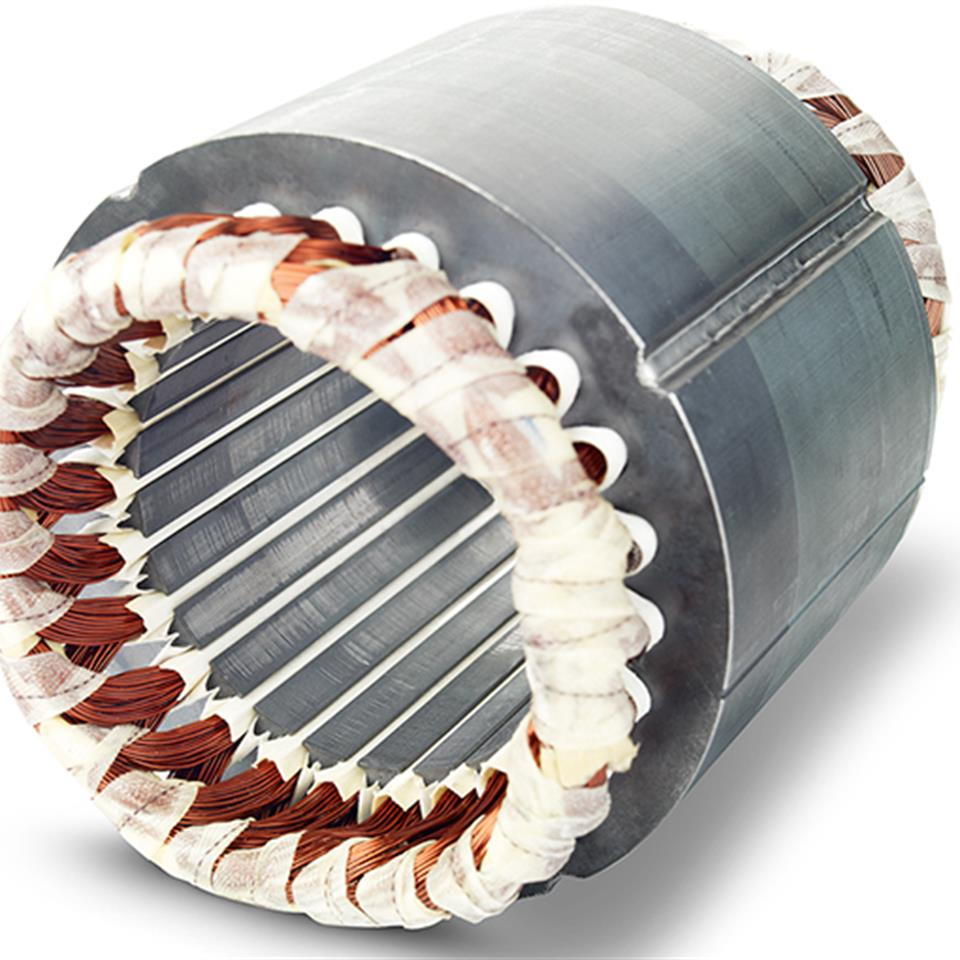
\includegraphics[scale=.1]{images-chude1/stator-1.jpg} 
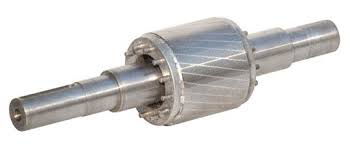
\includegraphics[scale=.3]{images-chude1/roto-long-soc.jpg}
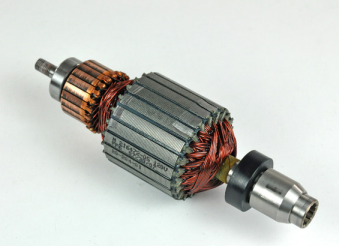
\includegraphics[scale=.4]{images-chude1/rotor-day-quan.png} 
\end{center}
\end{frame}

%--------------------------------------------------------------------------------
%--------------------------------------------------------------------------------
% Nguyen ly lam viec cua dong co khong dong bo
\section[Nguyên lý hoạt động]{Nguyên lý hoạt động động cơ không đồng bộ}
\begin{frame}{Nguyên lý hoạt động của ĐC KĐB}
\begin{columns}
\column{0.3\textwidth}
\vspace{-3cm}
\begin{center}
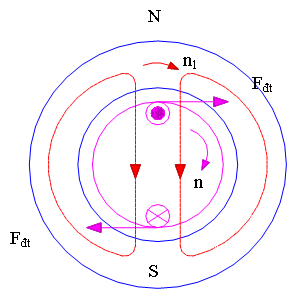
\includegraphics[scale=.5]{images-chude1/nguyenlylamviec.png} 
\end{center}
\column{0.6\textwidth}
- Dòng AC, $f_1$ qua dây quấn stator $\rightarrow$ từ trường $n_1$ $\rightarrow$ cắt thanh dẫn của rotor, và cảm ứng suất điện động.

- Dòng trong thanh dẫn rotor (dây quấn rotor ngắn mạch) kết hợp với từ trường quay của máy $\rightarrow$ rotor quay theo chiều từ trường $n$.
\end{columns}
\end{frame}

%--------------------------------------------------------------------------------
%--------------------------------------------------------------------------------
% Cac phuong phap khoi dong
\section[Các phương pháp khởi động]{Các phương pháp khởi động động cơ không đồng bộ}
\begin{frame}[t]{Yêu cầu khi khởi động động cơ}
\justifying
\begin{itemize}
\item Có moment khởi động đủ lớn.
\item Dòng khởi động nhỏ.
\item Phương pháp khởi động dùng thiết bị đơn giản, rẻ tiền và chắc chắn.
\item Tổn hao công suất trong quá trình khởi động nhỏ.
\end{itemize}
\end{frame}

\begin{frame}{Các phương pháp khởi động động cơ không đồng bộ ba pha}
\begin{itemize}
\item Khởi động trực tiếp.
\item Khởi động sao -- tam giác.
\item Khởi động dùng máy biến áp tự ngẫu.
\item Khởi động dùng cuộn kháng phụ (hoặc điện trở phụ) cho mạch stator hoặc mạch rotor.
\item Khởi động mềm.
%\item Khởi động part-winding.
\end{itemize}
\end{frame}

%--------------------------------------------------------------------------------
%--------------------------------------------------------------------------------
% Khoi dong truc tiep
\subsection*{Khởi động trực tiếp}

\begin{frame}{Khởi động trực tiếp}{Mạch động lực và mạch điều khiển}
	\vspace{-.5cm}
	\begin{center}
		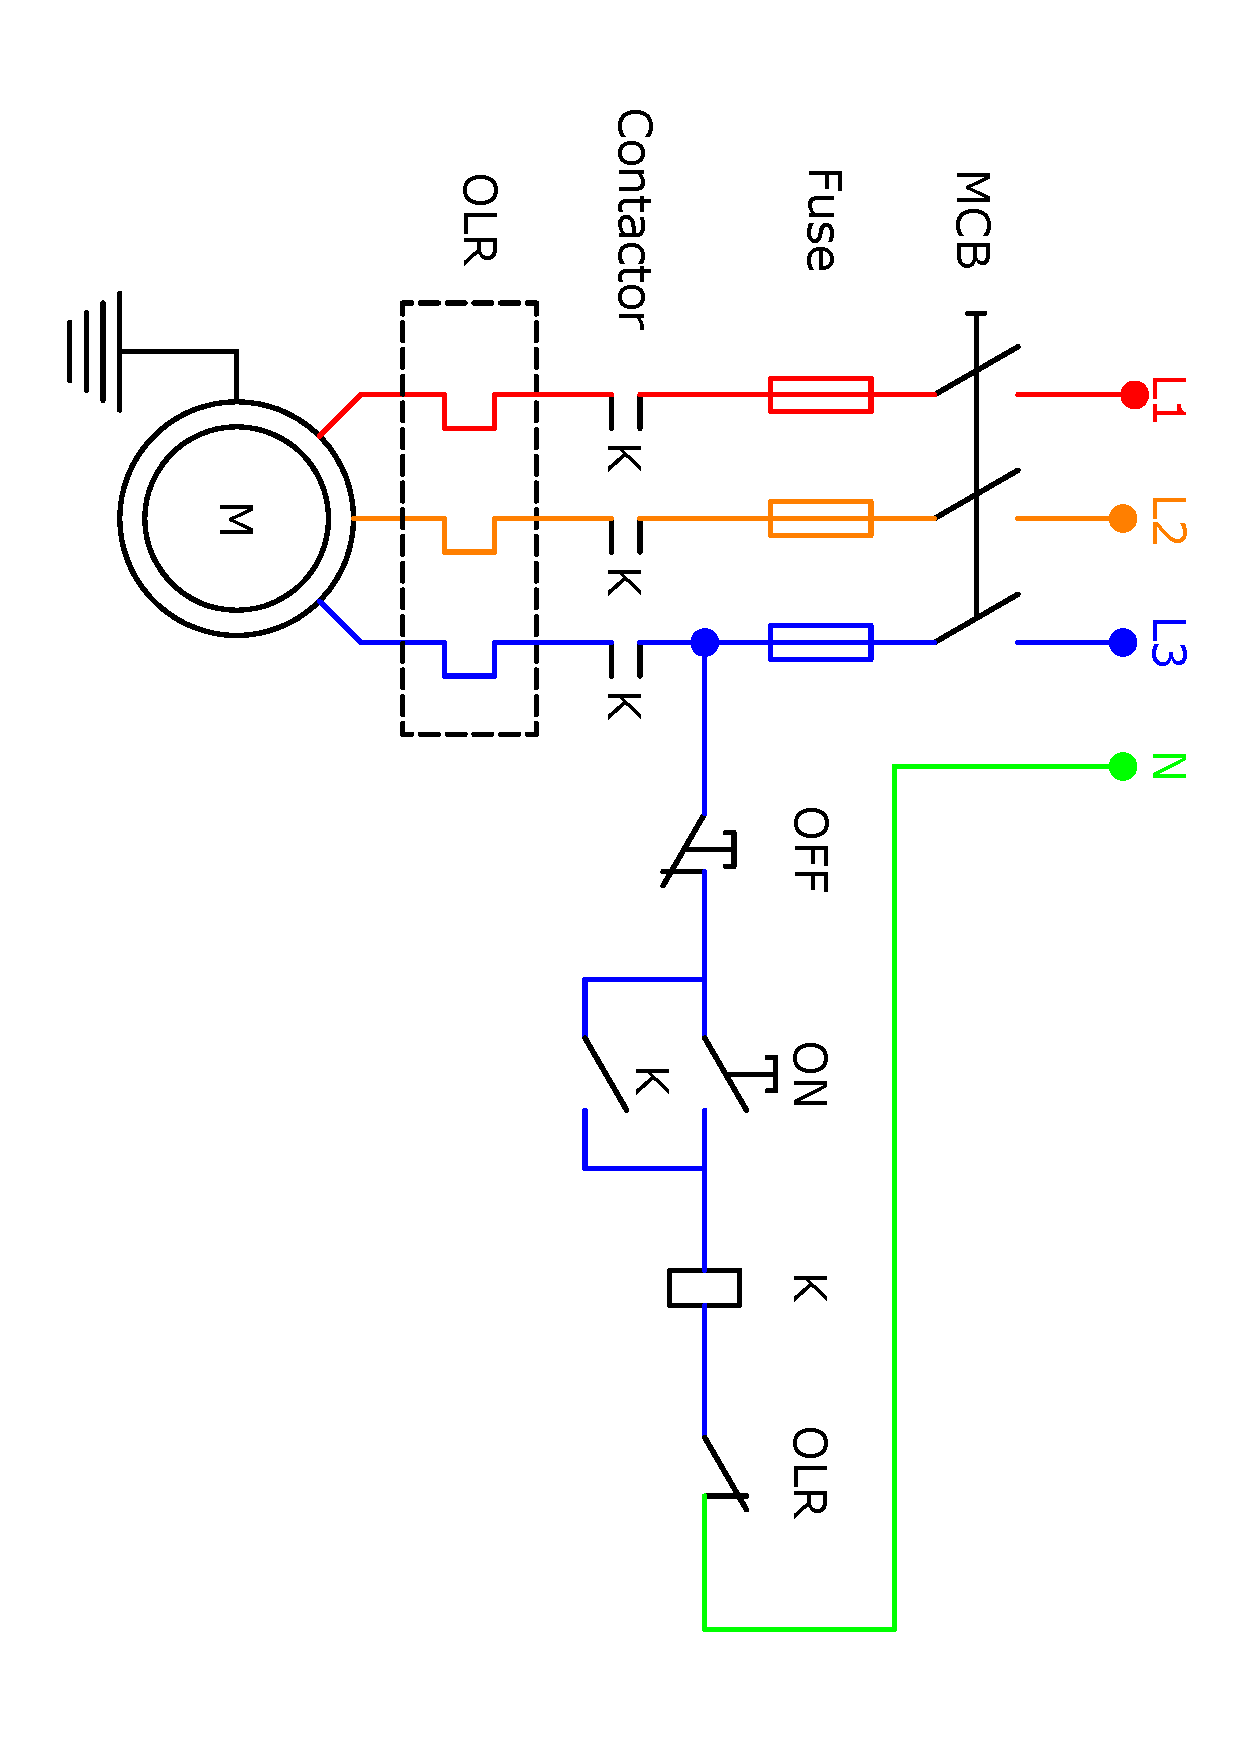
\includegraphics[width = 0.6\textwidth,angle=90]{../sodomach/sodomach-bc-chude1-1.pdf}
	\end{center}
\end{frame}


\begin{frame}{Khởi động trực tiếp}{Đặc tính moment của động cơ}
\vspace{-.6cm}
\begin{center}
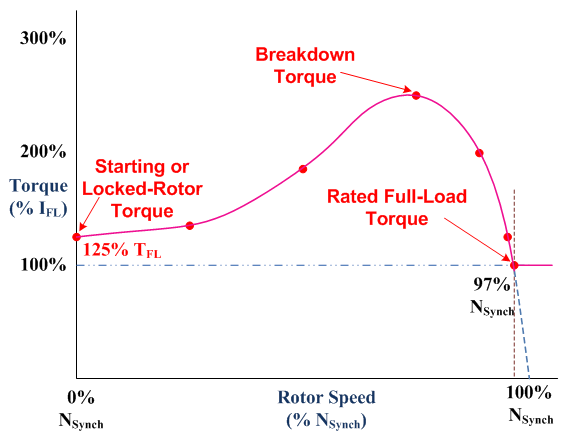
\includegraphics[scale=.58]{images-chude1/moment-tocdo.png} 
\end{center}
\end{frame}

\begin{frame}{Khởi động trực tiếp}{Ưu, nhược điểm và ứng dụng}
	\vspace{-1cm}
	\begin{columns}
	\column{0.65\textwidth}
		\begin{center}
			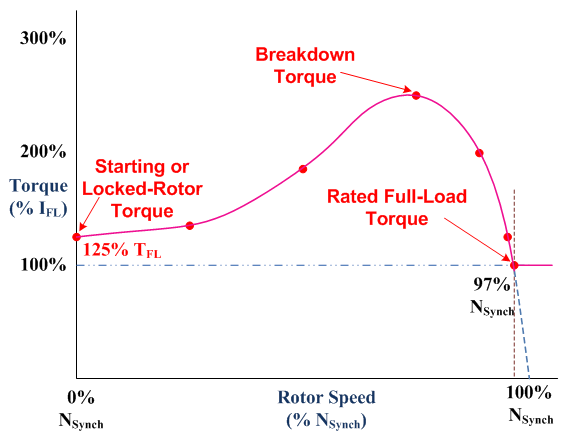
\includegraphics[scale=.5]{images-chude1/moment-tocdo.png} 
		\end{center}
		
		\column{0.45\textwidth}
		\begin{block}{Ưu điểm}
			\begin{itemize}
				\item Moment khởi động lớn.
				\item Sơ đồ đơn giản.
				\item Chi phí thấp.
			\end{itemize}
		\end{block}
	\end{columns}
\end{frame}

\begin{frame}{Khởi động trực tiếp}{Đặc tính dòng khởi động của động cơ}
\vspace{-.5cm}
\begin{center}
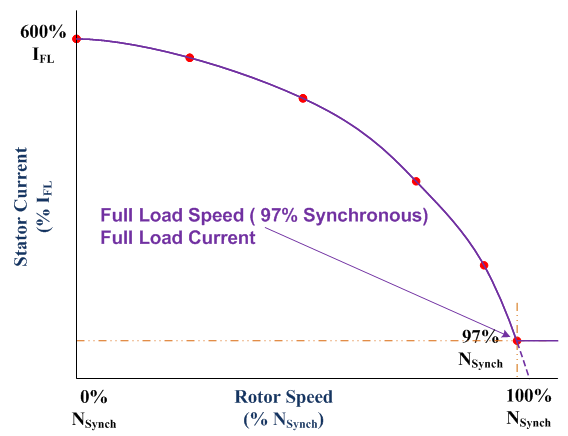
\includegraphics[scale=.58]{images-chude1/dongdien-tocdo.png} 
\end{center}
\end{frame}


\begin{frame}{Khởi động trực tiếp}{Ưu, nhược điểm và ứng dụng}
\vspace{-.5cm}
\begin{columns}

\column{0.65\textwidth}
\begin{center}
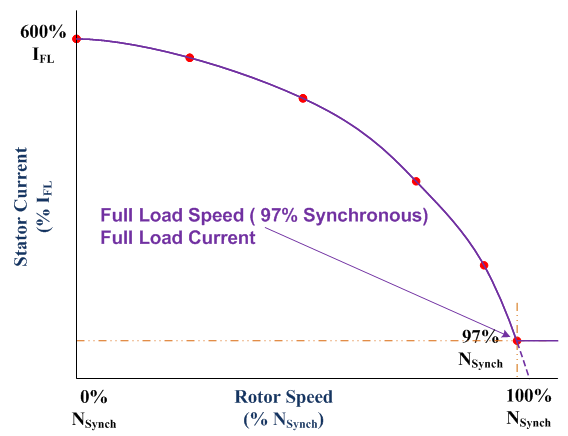
\includegraphics[scale=.5]{images-chude1/dongdien-tocdo.png} 
\end{center}
\column{0.45\textwidth}
\begin{small}	
\begin{block}{Nhược điểm}
\begin{itemize}
\item Dòng khởi động lớn, gây sụt áp.
\item Đông cơ chạy không êm.
\end{itemize}
\end{block}			
\begin{block}{Ứng dụng}
Cho ứng dụng có lực quán tính nhỏ.
\end{block}
\end{small}
\end{columns}
\end{frame}

%--------------------------------------------------------------------------------
%--------------------------------------------------------------------------------
% Khoi dong sao - tam giac
\subsection*{Khởi động sao -- tam giác}
\begin{frame}{Khởi động sao -- tam giác}{Mạch động lực và mạch điều khiển}
	\vspace{-.9cm}
	\begin{center}
		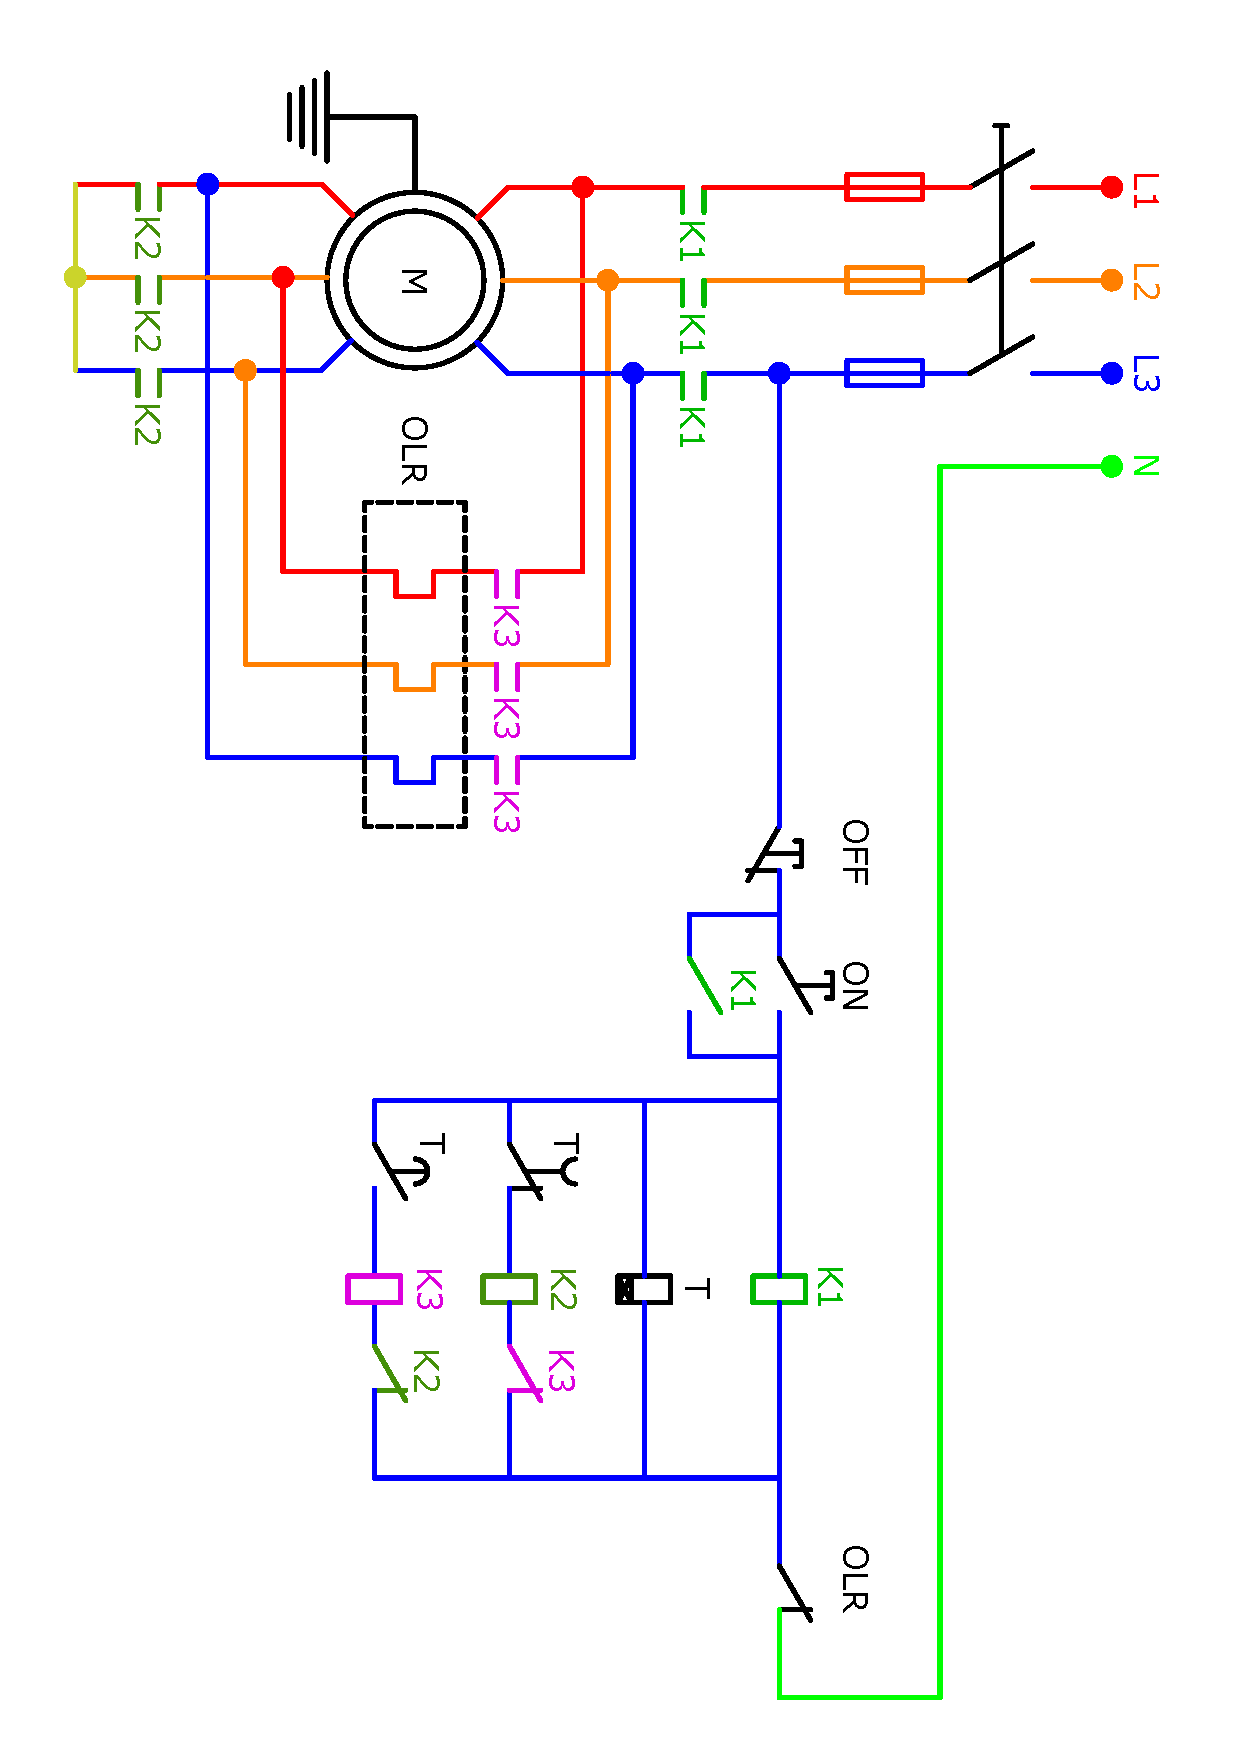
\includegraphics[width = 0.65\textwidth,angle=90]{../sodomach/sodomach-bc-chude1-2.pdf}
	\end{center}
\end{frame}

\begin{frame}{Khởi động sao -- tam giác}{Sự chuyển đổi sao -- tam giác}
	\vspace{-.5cm}
	\begin{center}
		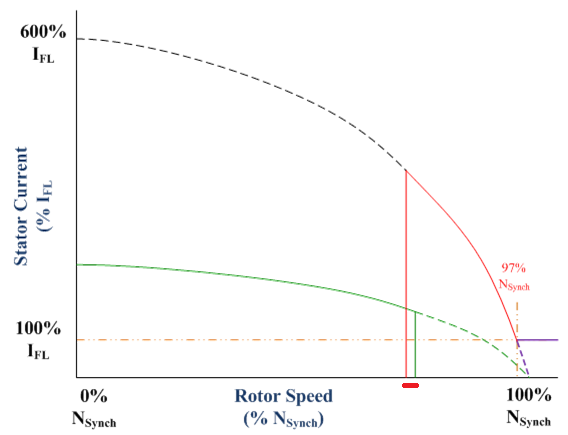
\includegraphics[scale=.5]{images-chude1/chuyentiep-sao-tam-giac.png} 
	\end{center}
\end{frame}

\begin{frame}{Khởi động sao -- tam giác}{Đặc tính dòng khởi động}
\vspace{-.5cm}
\begin{center}
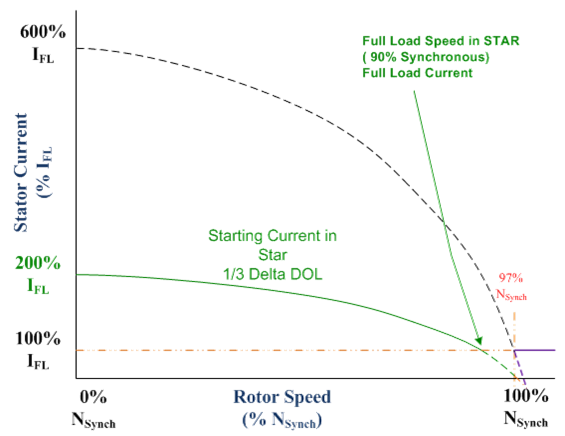
\includegraphics[scale=.5]{images-chude1/dongdien-sao.png} 
\end{center}
\end{frame}

\begin{frame}{Khởi động sao -- tam giác}{Ưu, nhược điểm và ứng dụng}
\begin{columns}

\column{0.65\textwidth}
\vspace{-1.5cm}
\begin{center}
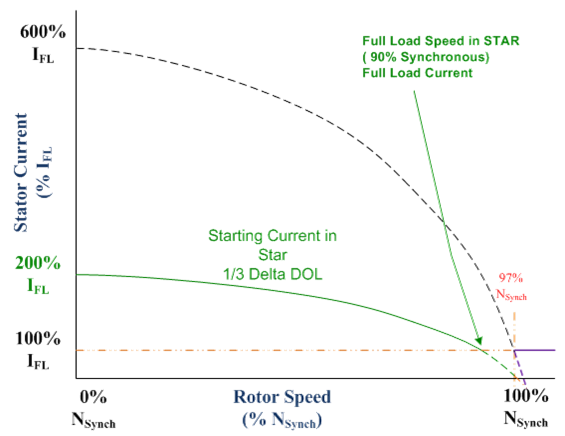
\includegraphics[scale=.4]{images-chude1/dongdien-sao.png} 
\end{center}
\column{0.4\textwidth}
\begin{small}	
\begin{block}{Ưu điểm}
\begin{itemize}
\item Dòng khởi động qua stator giảm đi $\sqrt{3}$.
\item Dòng qua lưới giảm đi $3$ lần.
\end{itemize}
\end{block}			
\end{small}
\end{columns}
\end{frame}

\begin{frame}{Khởi động sao -- tam giác}{Đặc tính của moment}
\vspace{-.5cm}
\begin{center}
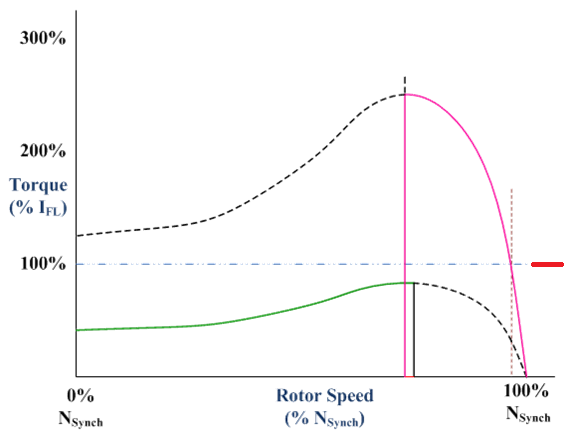
\includegraphics[scale=.47]{images-chude1/moment-sao-tamgiac.png} 
\end{center}
\end{frame}

\begin{frame}{Khởi động sao -- tam giác}{Ưu, nhược điểm và ứng dụng}
\begin{columns}

\column{0.65\textwidth}
\vspace{-1.5cm}
\begin{center}
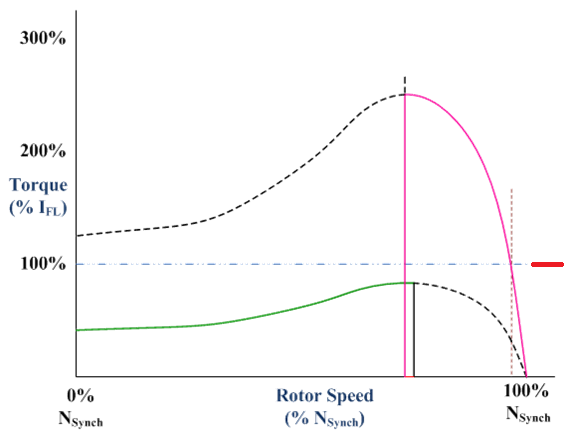
\includegraphics[scale=.45]{images-chude1/moment-sao-tamgiac.png} 
\end{center}
\column{0.4\textwidth}
\begin{small}	
\begin{block}{Nhược điểm}
Moment giảm đi $3$ lần.
\end{block}			
\begin{block}{Ứng dụng}
Dùng khởi động động cơ ở chế độ không tải: máy bơm, các máy trong ngành gỗ.
\end{block}
\end{small}
\end{columns}
\end{frame}

%--------------------------------------------------------------------------------
%--------------------------------------------------------------------------------
% Khoi dong bang may bien ap tu ngau
\subsection*{Khởi động dùng máy biến áp tự ngẫu}
\begin{frame}{Khởi động dùng MBA tự ngẫu}{Mạch động lực}
\vspace{-2.5cm}
\begin{center}
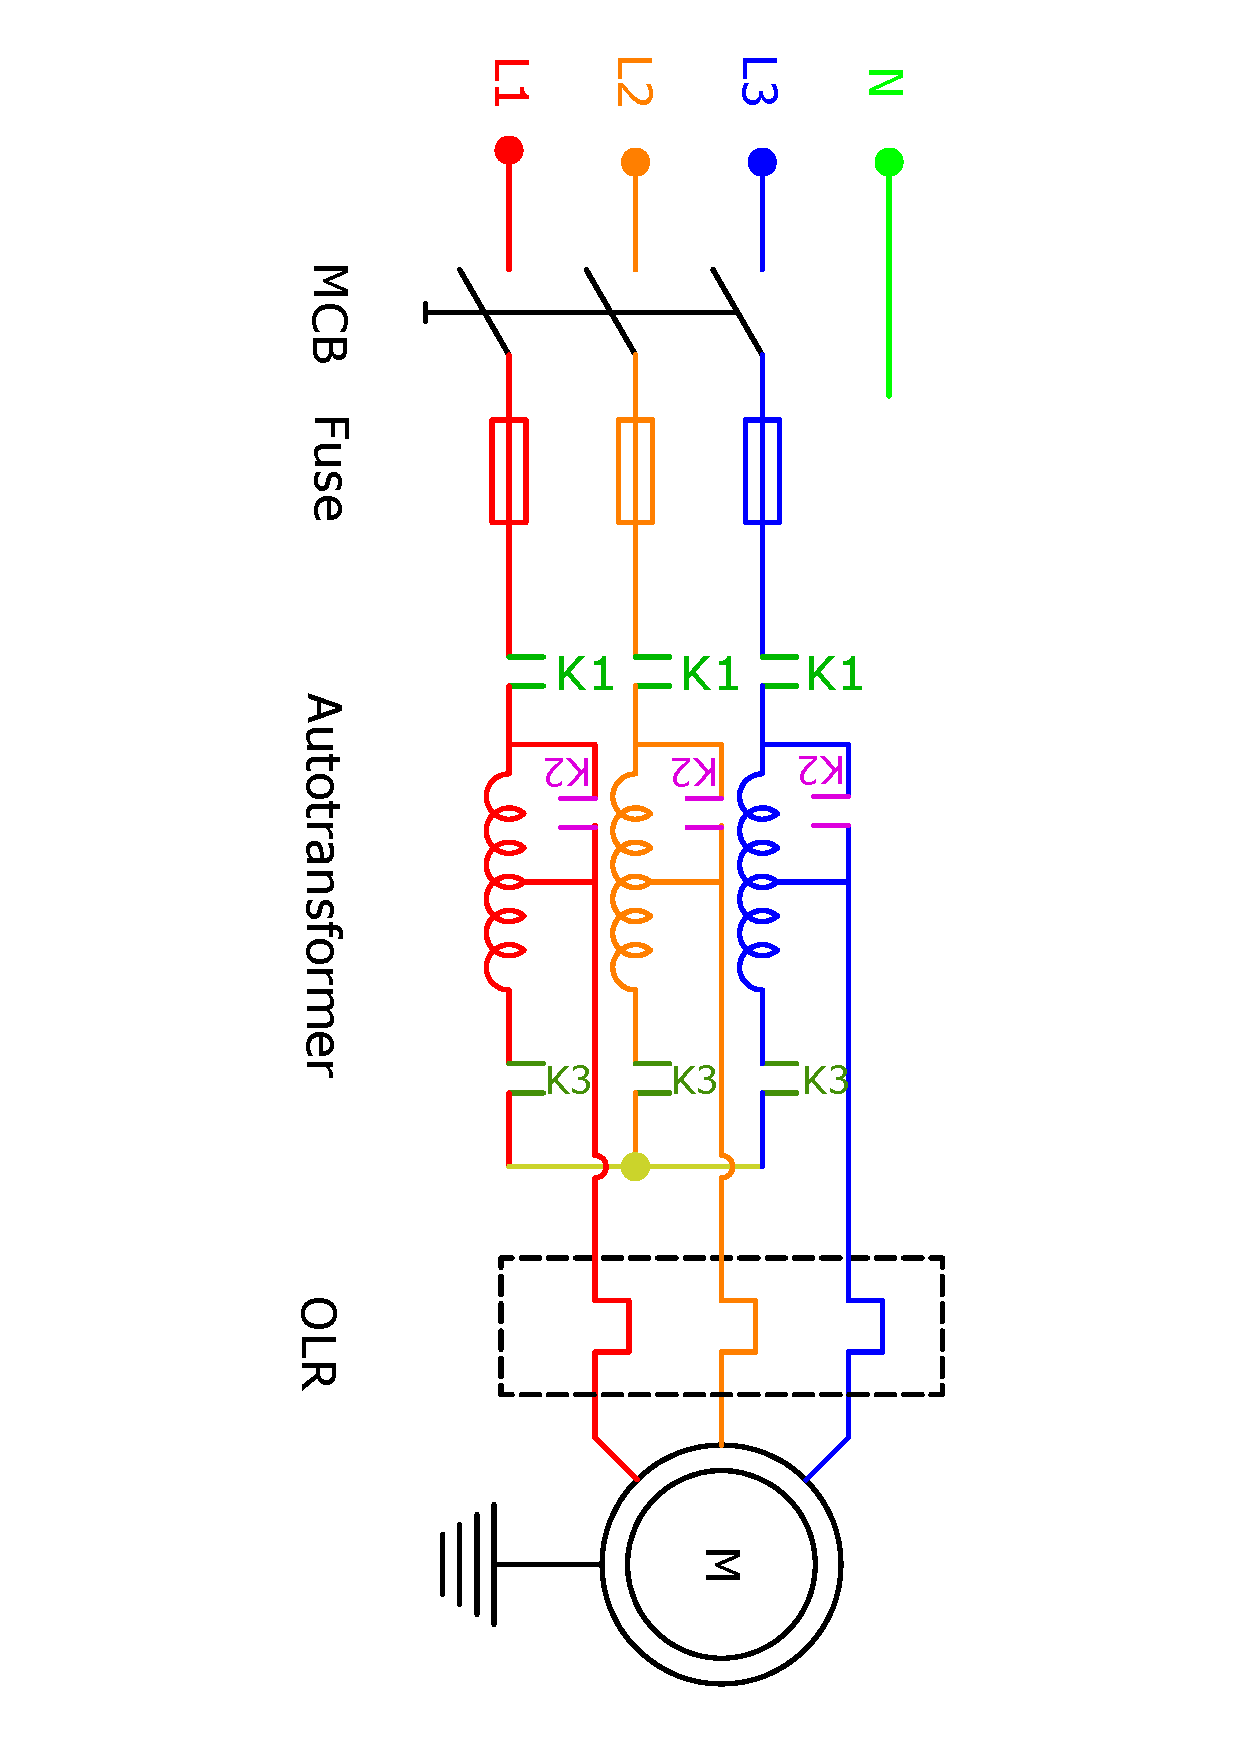
\includegraphics[width = 0.73\textwidth,angle=90]{../sodomach/sodomach-bc-chude1-3.pdf}
\end{center}
\end{frame}

\begin{frame}{Khởi động dùng MBA tự ngẫu}{Mạch điều khiển}
\vspace{-1.5cm}
\begin{center}
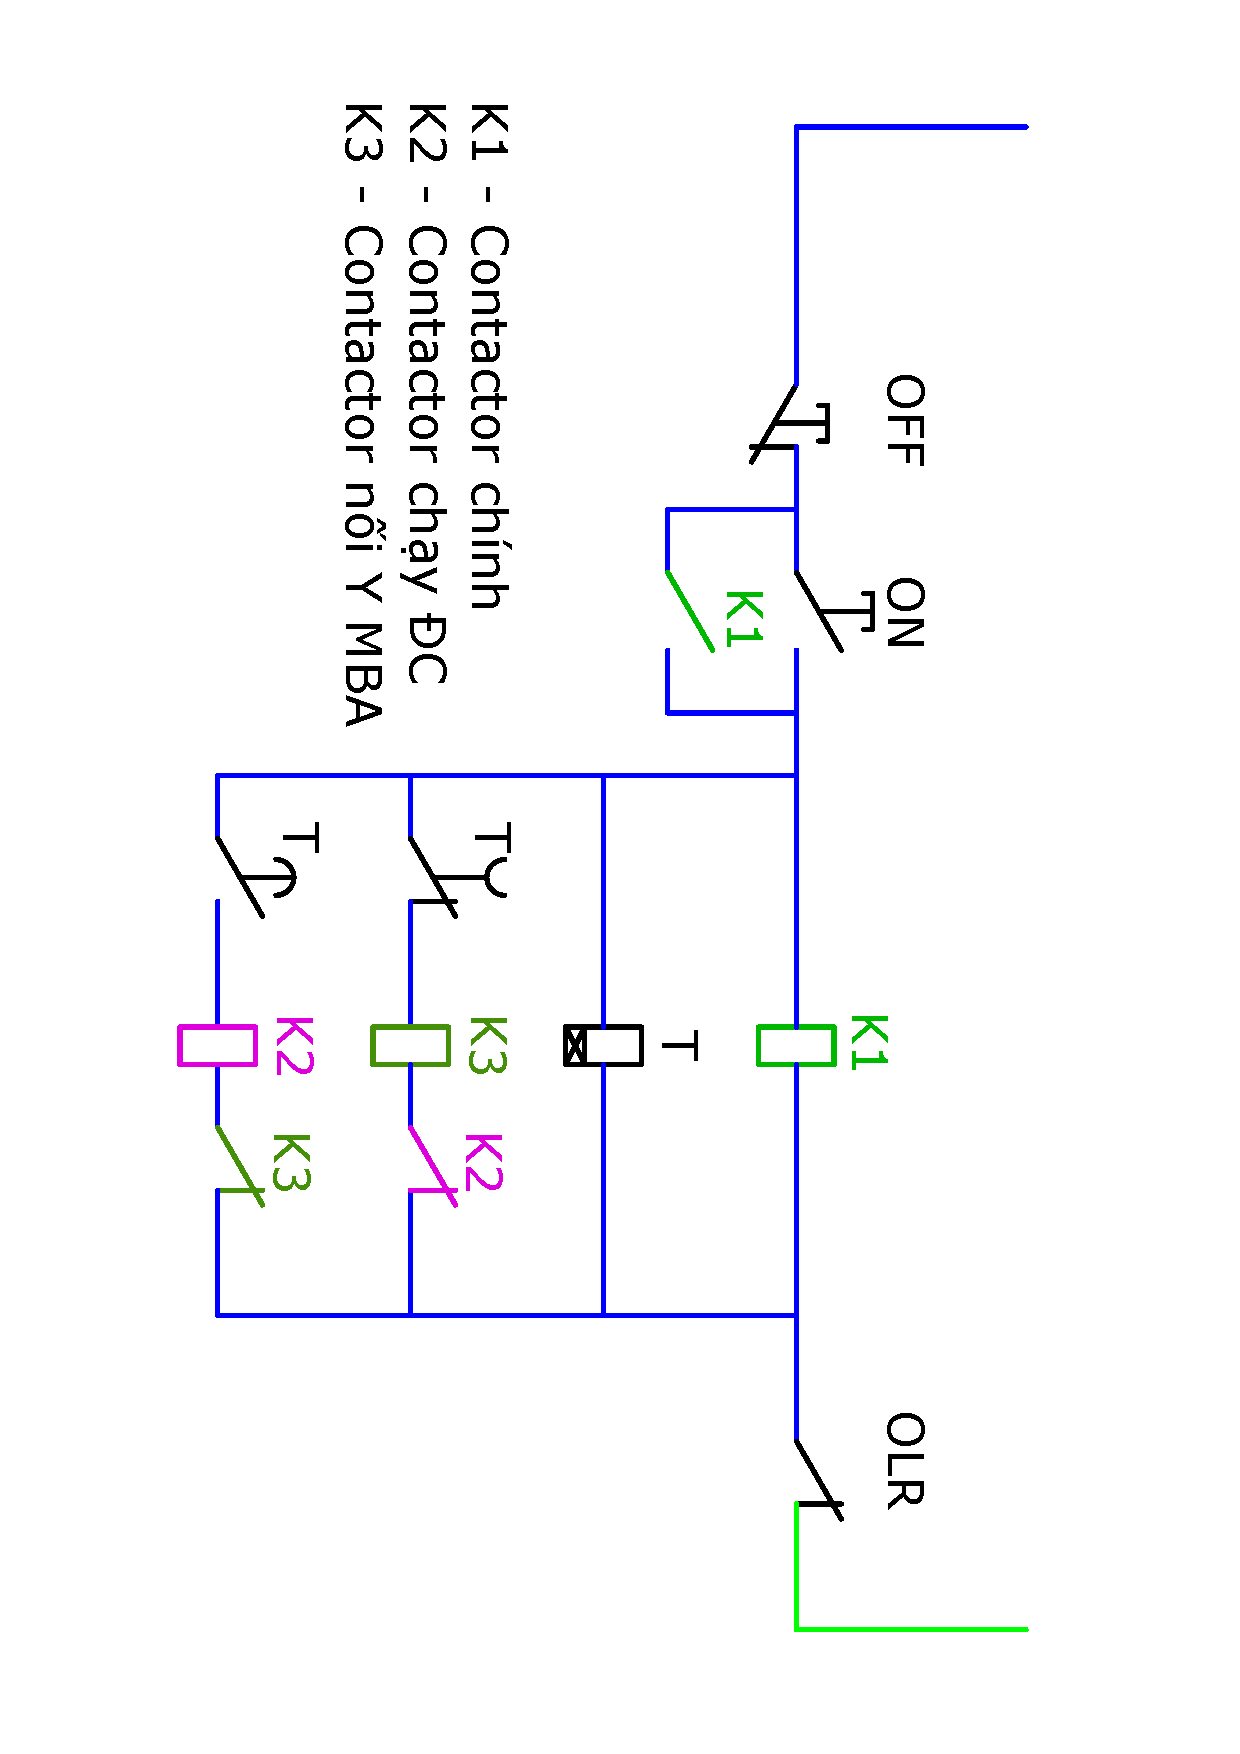
\includegraphics[width = 0.7\textwidth,angle=90]{../sodomach/sodomach-bc-chude1-34.pdf}
\end{center}
\end{frame}

\begin{frame}{Khởi động dùng MBA tự ngẫu}{Nguyên lý hoạt động}
\begin{enumerate}
\item Khởi động, $K1$ và $K3$ đóng.
\end{enumerate}
\vspace{-2.5cm}
\begin{center}
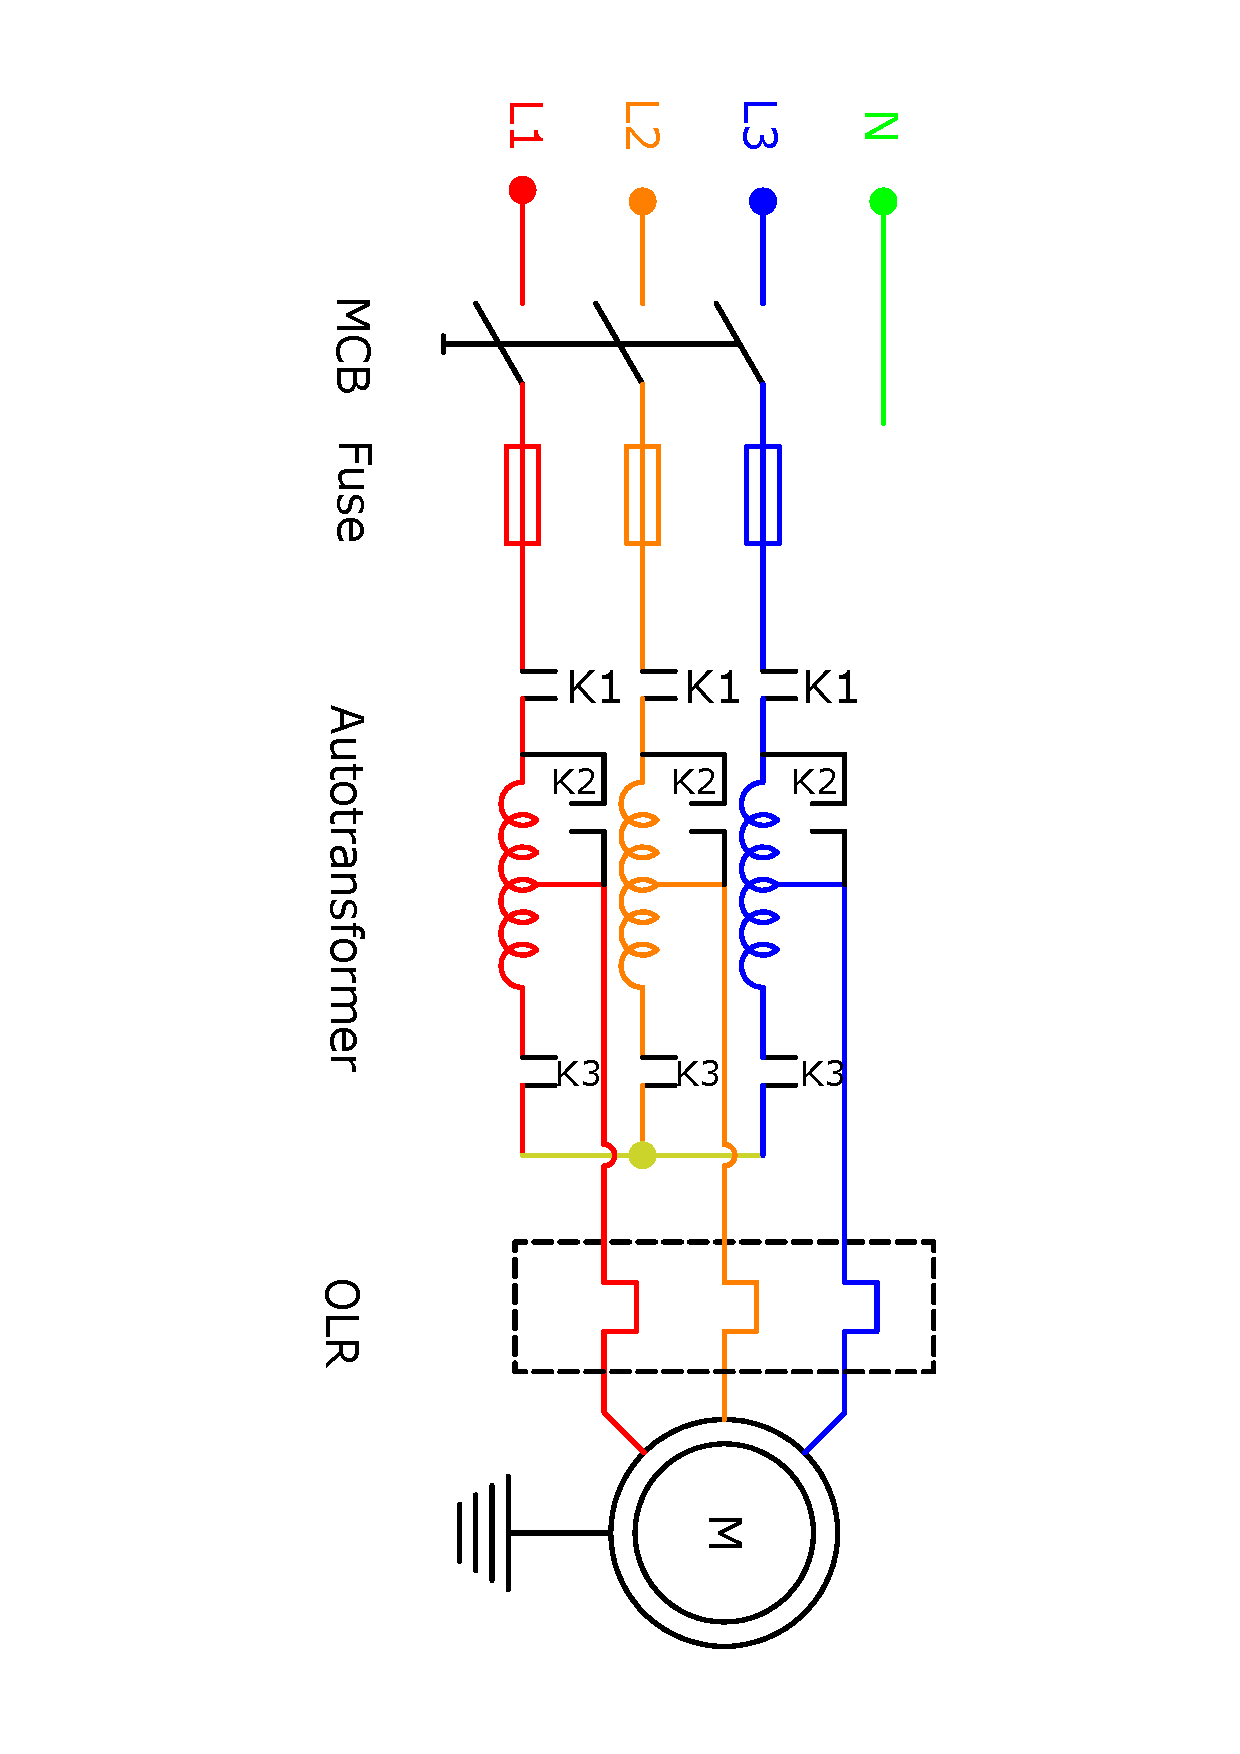
\includegraphics[width = 0.73\textwidth,angle=90]{../sodomach/sodomach-bc-chude1-31.pdf}
\end{center}
\end{frame}

\begin{frame}{Khởi động dùng MBA tự ngẫu}{Nguyên lý hoạt động}
\begin{enumerate}
\setcounter{enumi}{1}
\item Sau một thời gian, $K3$ ngắt ra.
\end{enumerate}
\vspace{-2.5cm}
\begin{center}
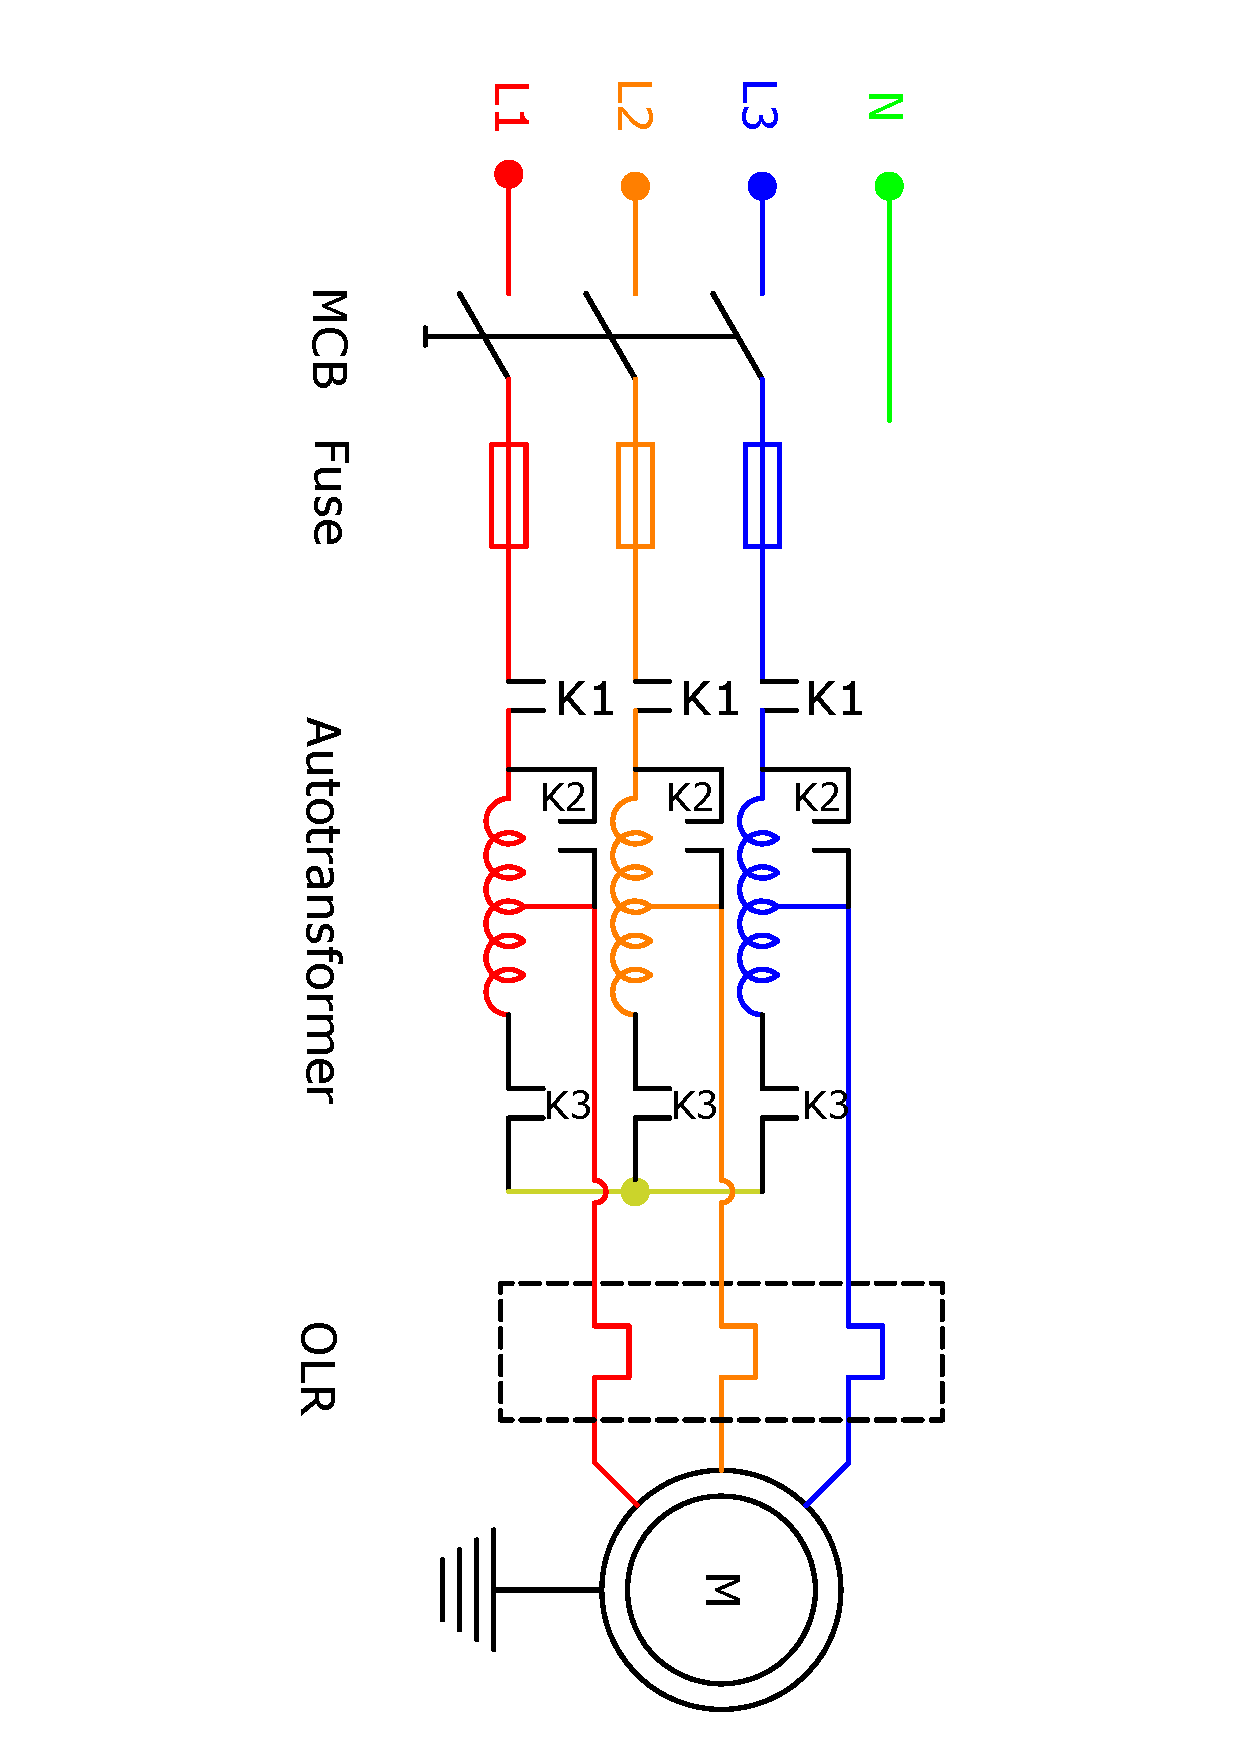
\includegraphics[width = 0.73\textwidth,angle=90]{../sodomach/sodomach-bc-chude1-32.pdf}
\end{center}
\end{frame}

\begin{frame}{Khởi động dùng MBA tự ngẫu}{Nguyên lý hoạt động}
\begin{enumerate}
\setcounter{enumi}{2}
\item Đóng $K2$.
\end{enumerate}
\vspace{-2.5cm}
\begin{center}
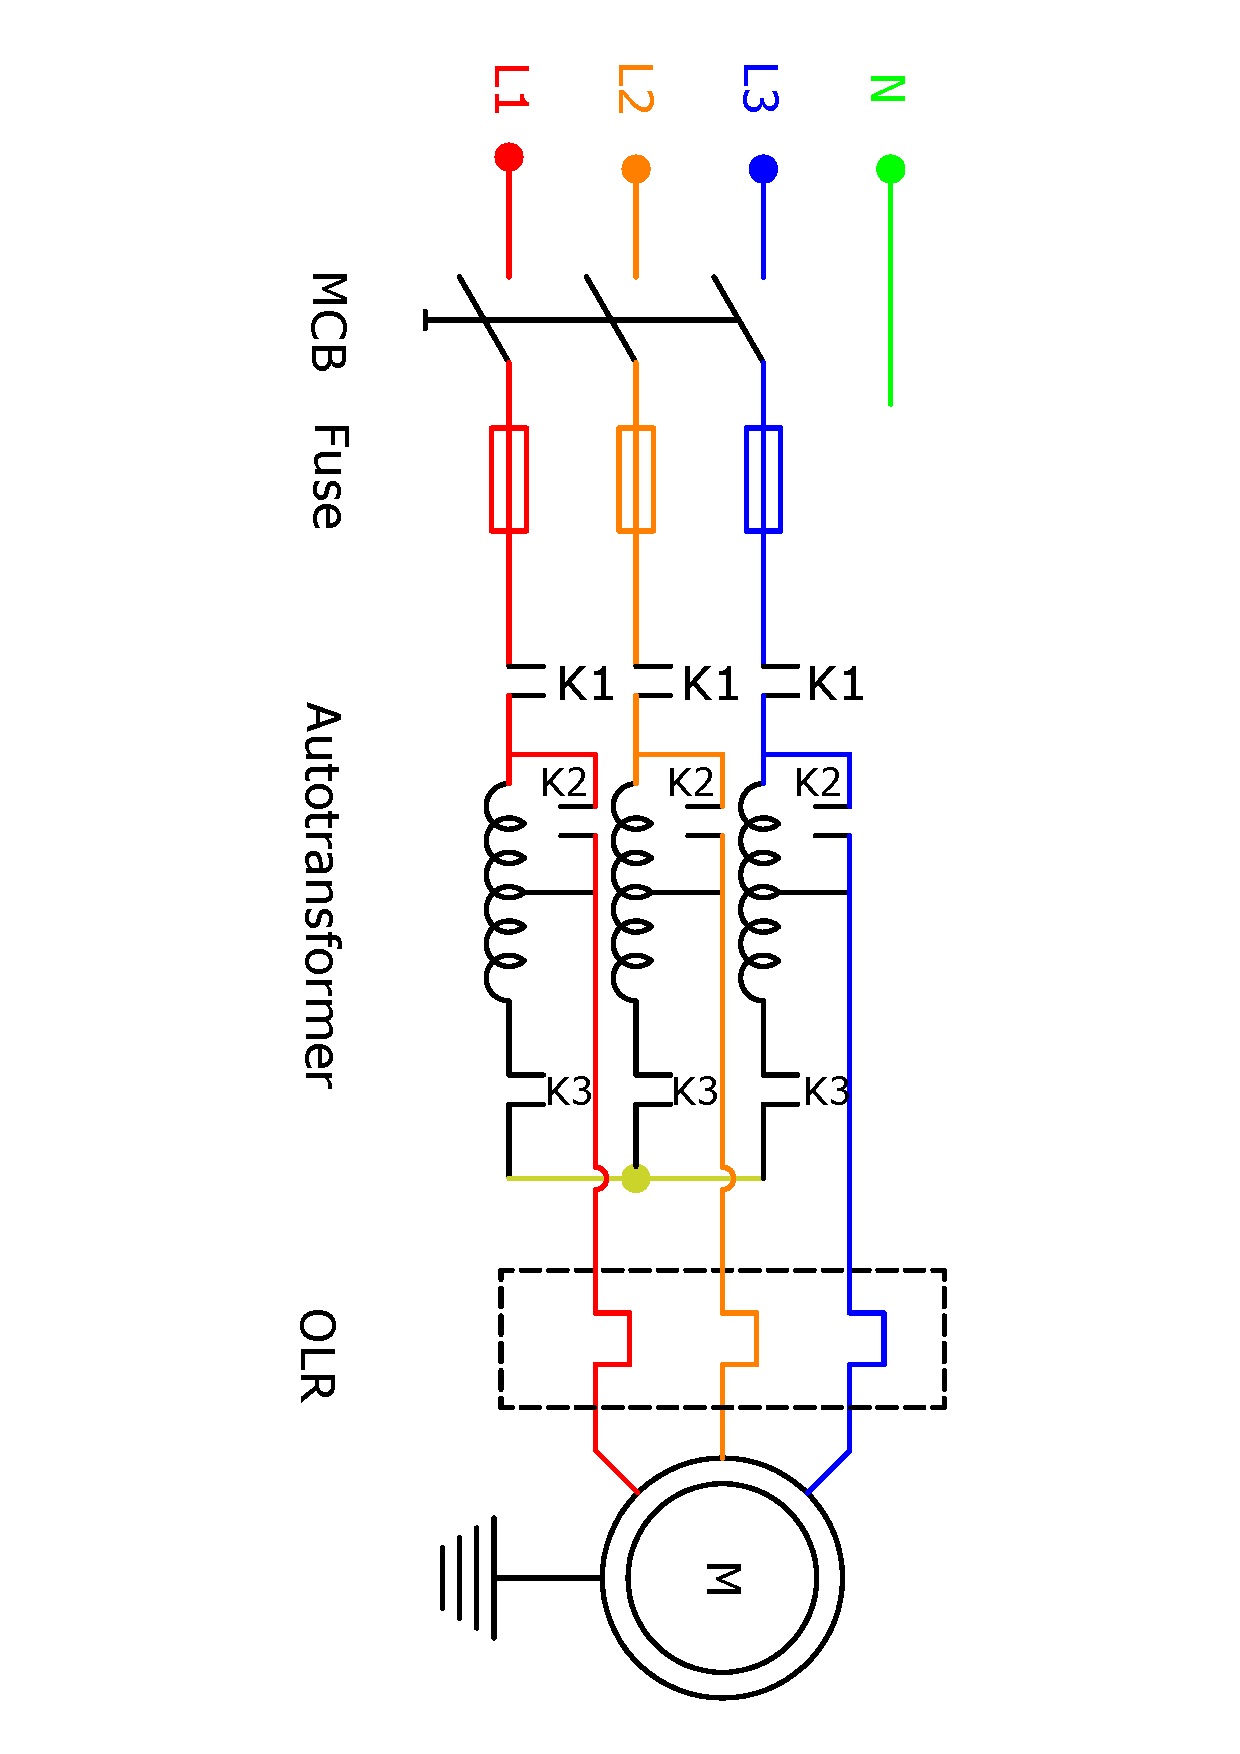
\includegraphics[width = 0.73\textwidth,angle=90]{../sodomach/sodomach-bc-chude1-33.pdf}
\end{center}
\end{frame}

\begin{frame}[t]{Khởi động dùng MBA tự ngẫu}{Ưu, nhược điểm và ứng dụng}
\begin{itemize}
\item \alert{Ưu điểm}
\begin{itemize}
\item Lựa chọn được các giá trị điện áp, moment quay.
\item Khởi động được với tải trọng tương đối nặng.
\end{itemize}
\item \alert{Nhược điểm}: Chi phí đầu tư ban đầu cao.
\item \alert{Ứng dụng}: Bơm thủy lực, băng tải,\ldots
\end{itemize}
\end{frame}

%--------------------------------------------------------------------------------
%--------------------------------------------------------------------------------
% Khoi dong bang điện trở phụ cho mạch stator
\subsection*{Dùng trở kháng phụ cho mạch stator}
\begin{frame}{Khởi động dùng điện trở phụ cho mạch stator}{Mạch động lực}
\vspace{-2.5cm}
\begin{center}
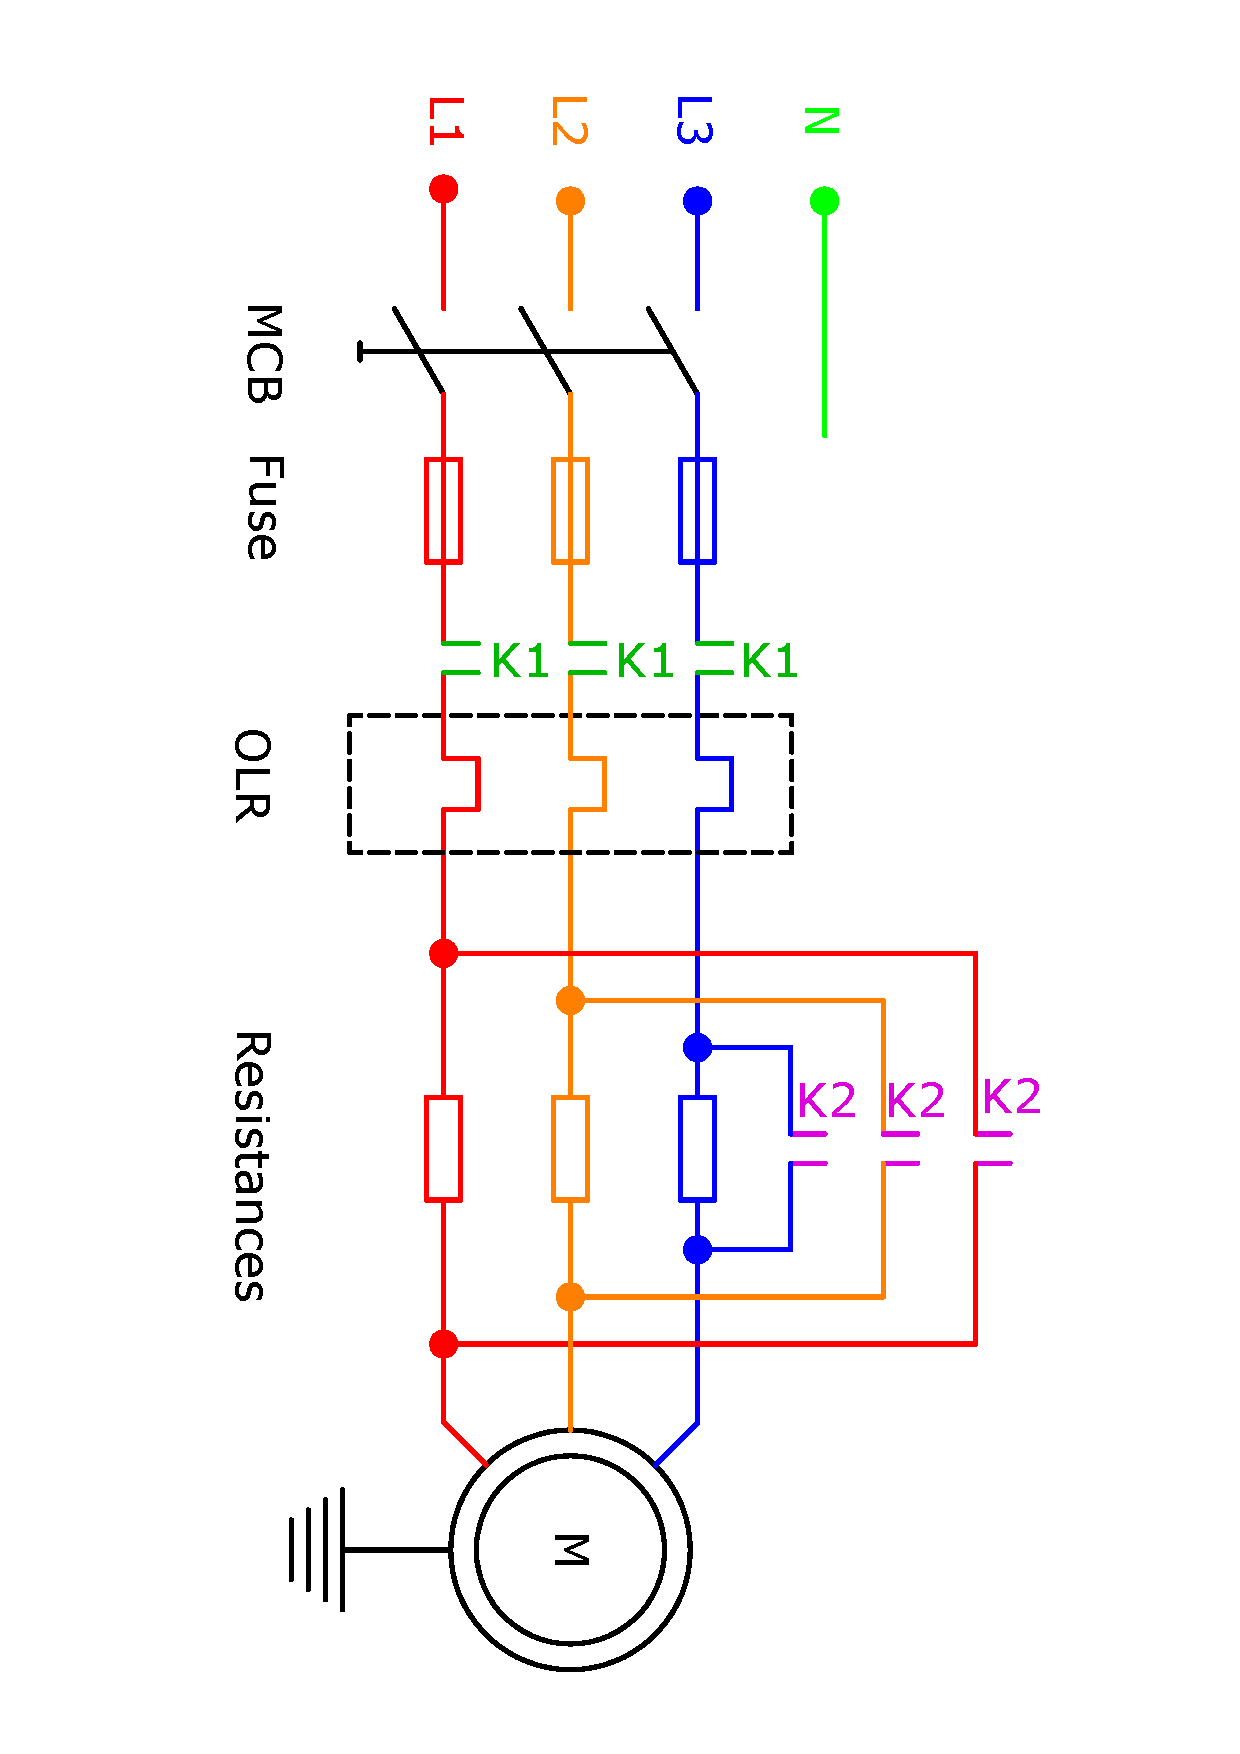
\includegraphics[width = 0.73\textwidth,angle=90]{../sodomach/sodomach-bc-chude1-4.pdf}
\end{center}
\end{frame}

\begin{frame}{Khởi động dùng điện trở phụ cho mạch stator}{Mạch điều khiển}
\vspace{-2cm}
\begin{center}
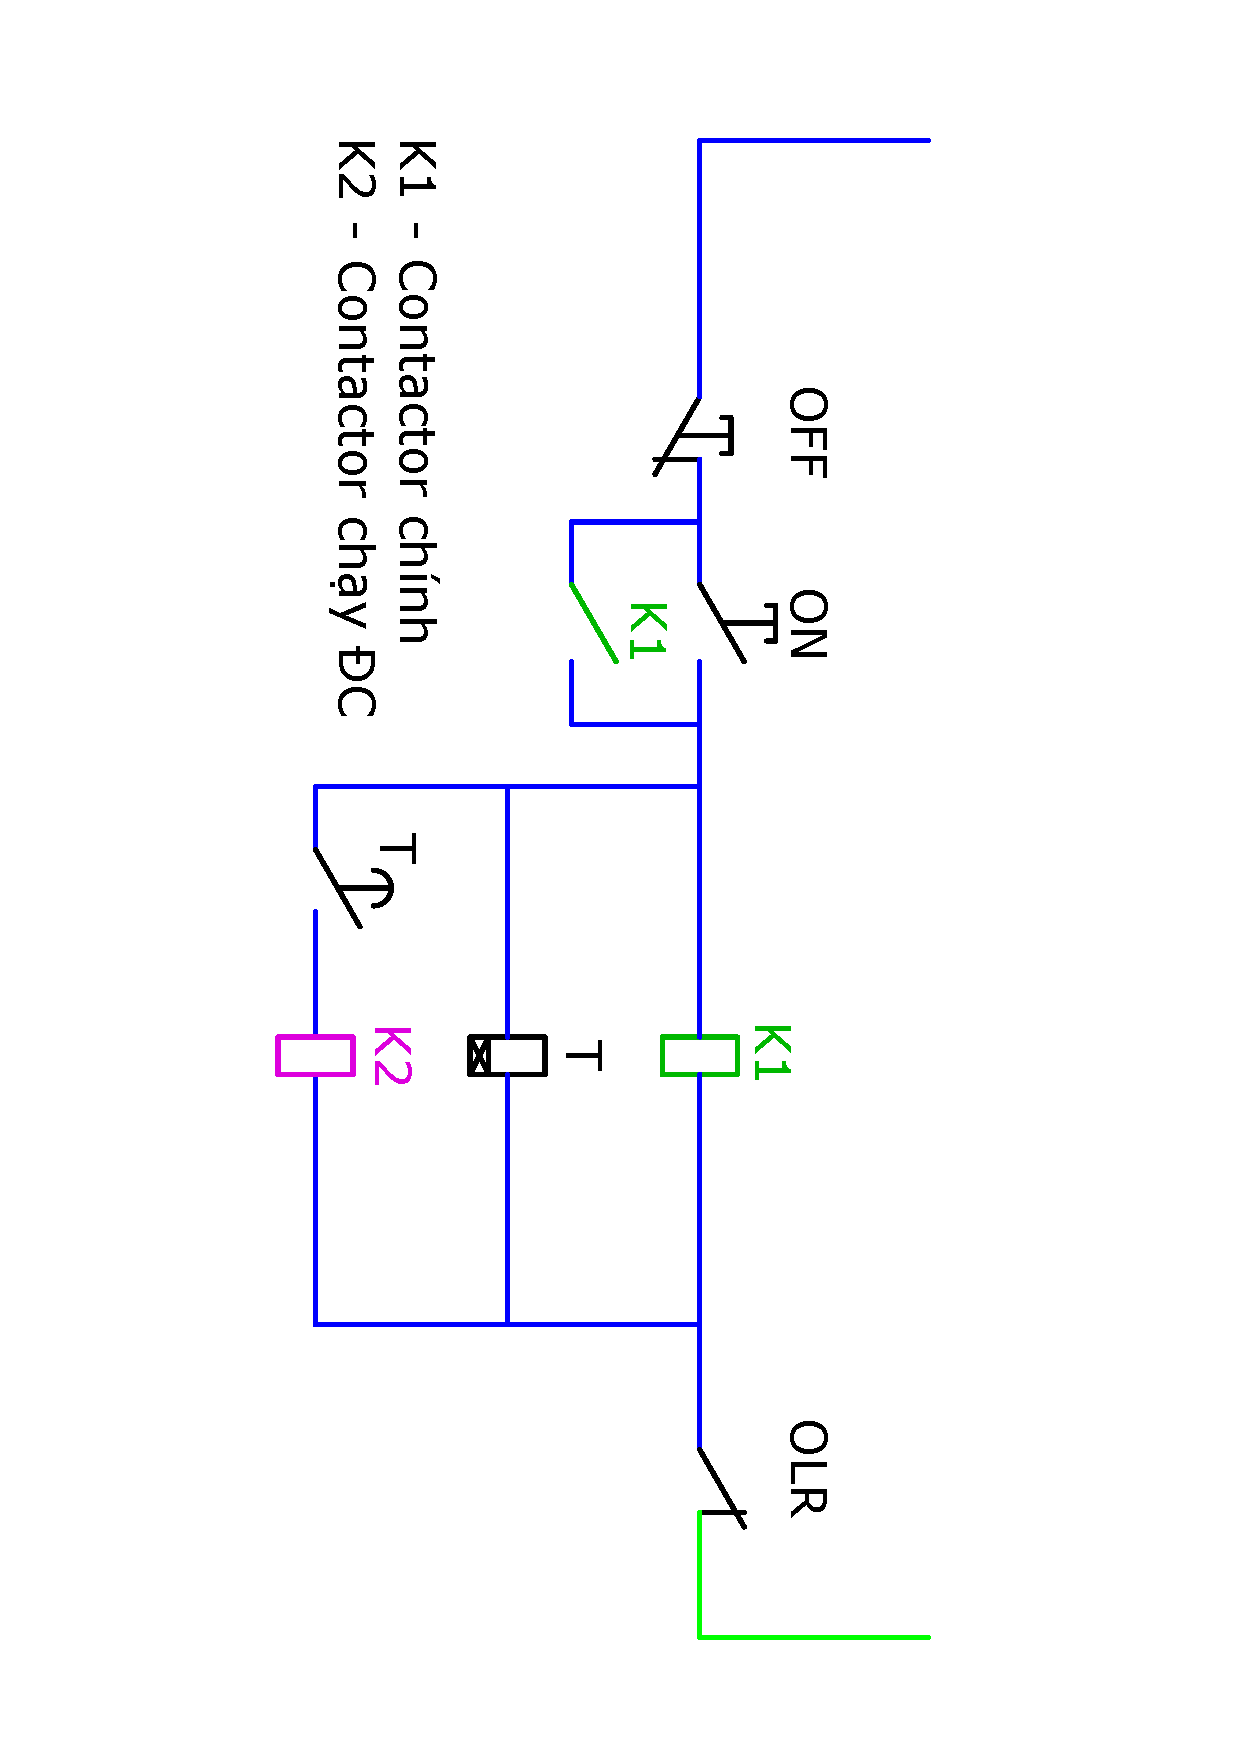
\includegraphics[width = 0.7\textwidth,angle=90]{../sodomach/sodomach-bc-chude1-41.pdf}
\end{center}
\end{frame}

\begin{frame}{Dùng điện trở phụ cho mạch stator}{Ưu, nhược điểm và ứng dụng}
\begin{itemize}
\item \alert{Ưu điểm}: Giảm dòng khởi động, tăng tốc êm.
\item \alert{Nhược điểm}: 
\begin{itemize}
\item Moment khởi động nhỏ, hiệu suất thấp, chi phí cao.
\item Dòng khởi động lớn hơn so với khởi động $Y - \Delta$.
\end{itemize}
\item \alert{Ứng dụng}: quạt, bơm ly tâm,\ldots
\end{itemize}
\end{frame}

%--------------------------------------------------------------------------------
%--------------------------------------------------------------------------------
% Khoi dong bang điện trở phụ cho mạch rotor
\subsection*{Dùng trở kháng phụ cho mạch rotor}
\begin{frame}{Khởi động dùng điện trở phụ cho mạch rotor}{Mạch động lực}
\vspace{-3cm}
\begin{center}
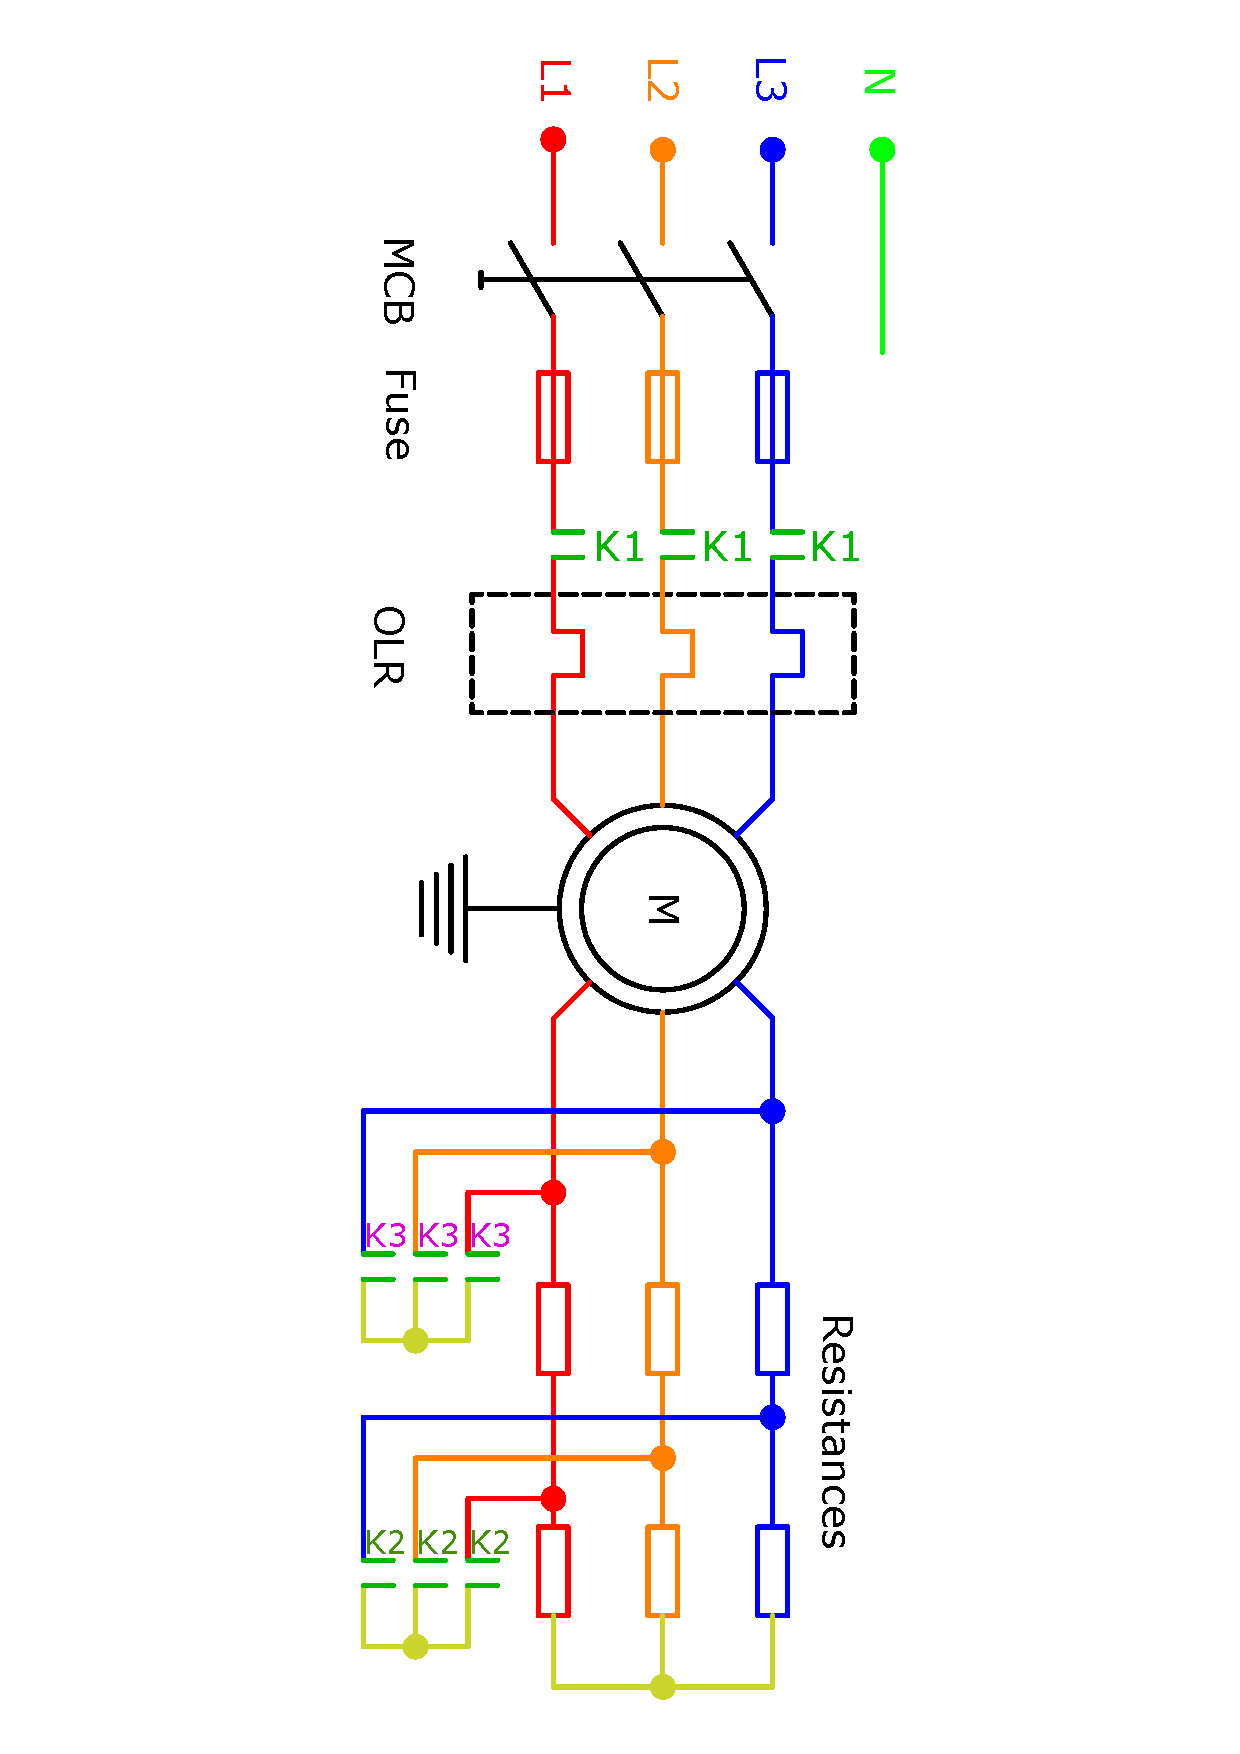
\includegraphics[width = 0.75\textwidth,angle=90]{../sodomach/sodomach-bc-chude1-5.pdf}
\end{center}
\end{frame}

\begin{frame}{KĐ dùng điện trở phụ cho mạch rotor}{Mạch điều khiển}
\vspace{-1cm}
\begin{center}
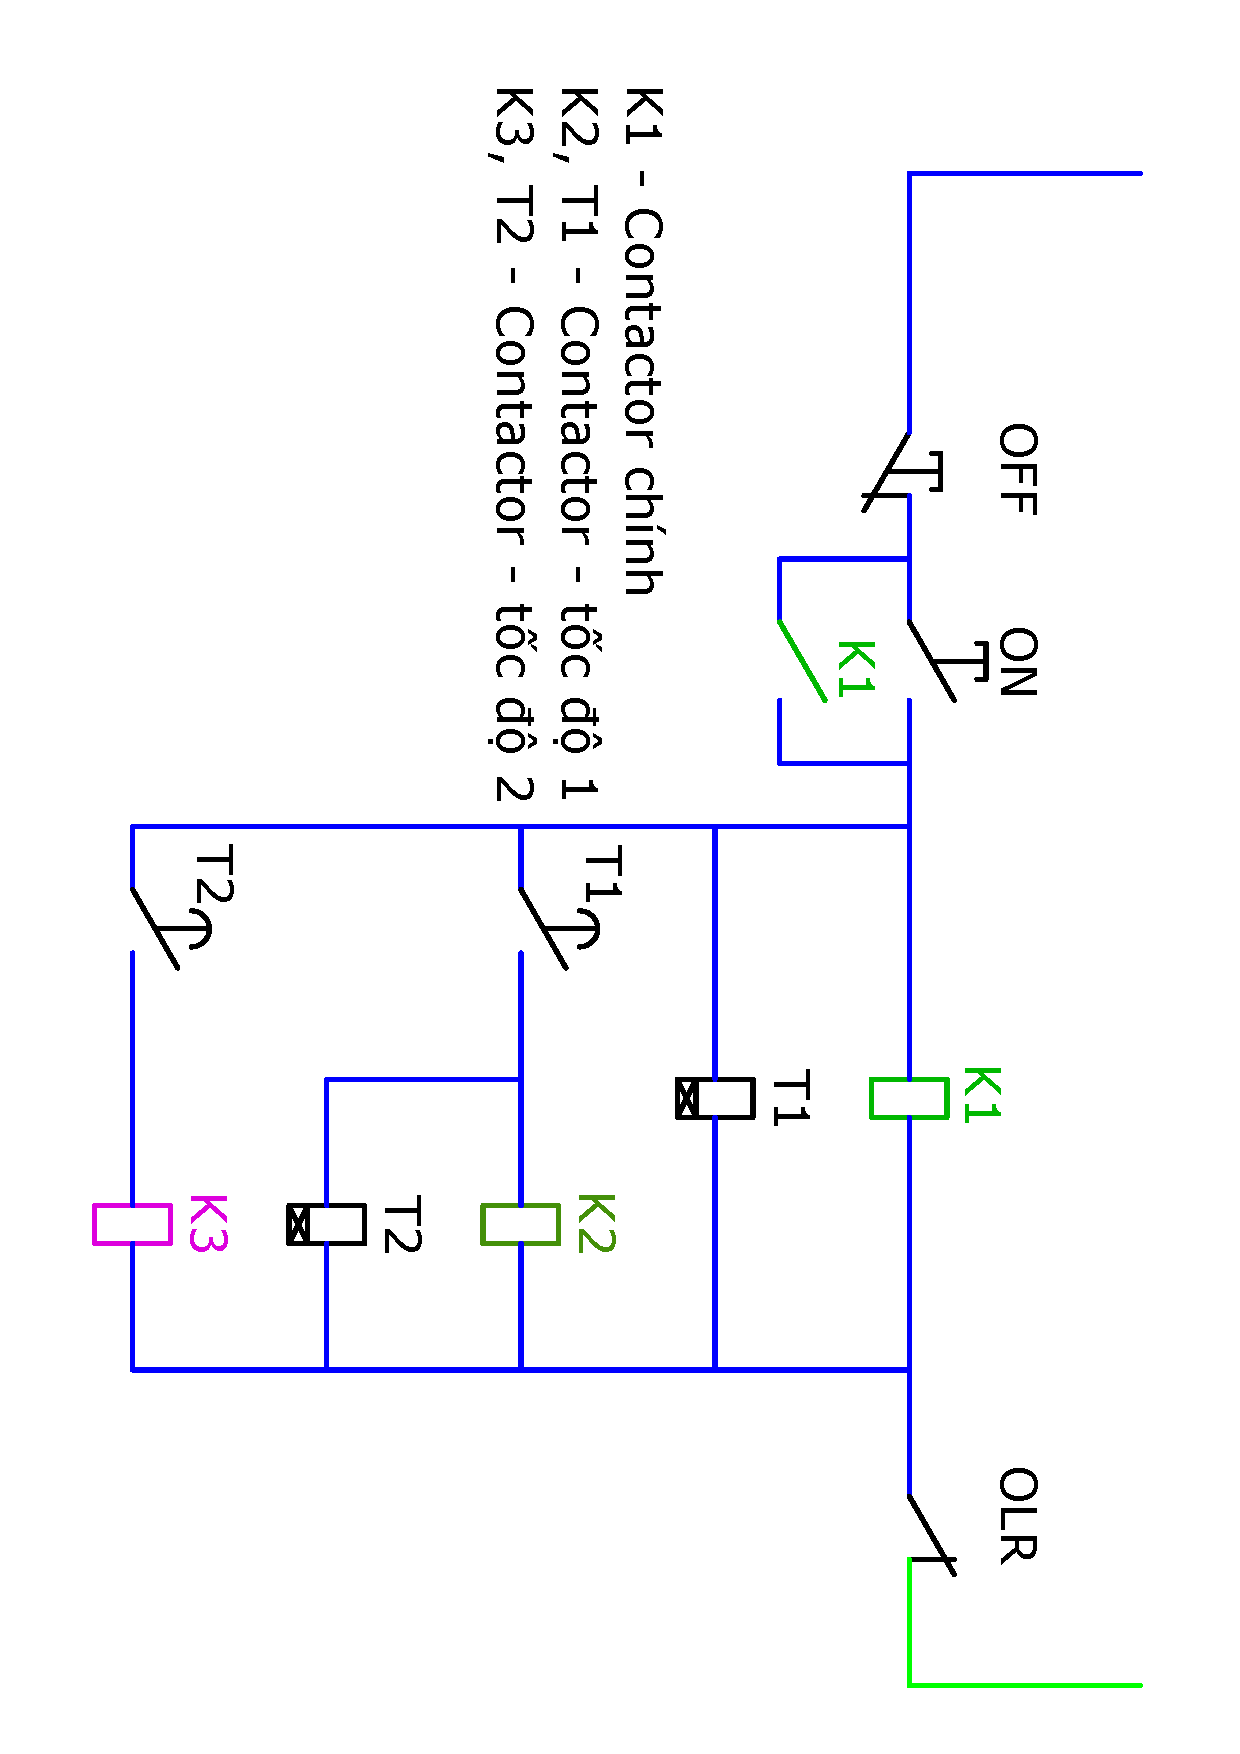
\includegraphics[width = 0.55\textwidth,angle=90]{../sodomach/sodomach-bc-chude1-51.pdf}
\end{center}
\end{frame}

\begin{frame}{Dùng điện trở phụ cho mạch rotor}{Ưu, nhược điểm và ứng dụng}
\begin{itemize}
\item \alert{Ưu điểm}: Đặc tính moment tốt, tăng tốc êm.
\item \alert{Nhược điểm}: Đầu tư lớn, thực hiện công tác bảo trì.
\item \alert{Ứng dụng}: Dùng cho tải có quán tính lớn: máy nén, máy cắt,\ldots
\end{itemize}
\end{frame}

%--------------------------------------------------------------------------------
%--------------------------------------------------------------------------------
% Khoi dong mem
\subsection*{Khởi động mềm}
\begin{frame}{Khởi động mềm}{Đặc điểm}
\begin{columns}
\column{0.3\textwidth}
\vspace{-2cm}
\begin{center}
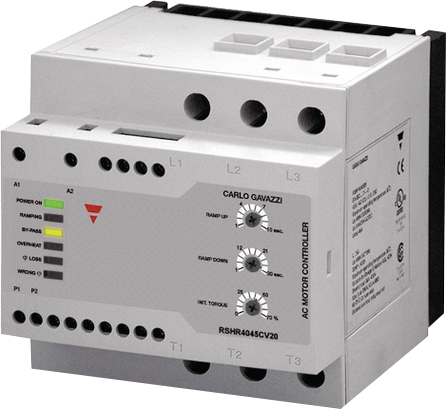
\includegraphics[scale=.25]{images-chude1/khoidongmem.png} 
\end{center}
\column{0.7\textwidth}
\begin{itemize}
\item Thay đổi điện áp (giữa nguyên tần số).
\item Điều chỉnh được chính xác lực khởi động mong muốn.
\item Điều khiển điện áp vào stator thông qua các $SCR$.
\end{itemize}
\end{columns}
\end{frame}
\begin{frame}{Khởi động mềm}{Mạch biển đổi điện áp}
\vspace{-1cm}
\begin{center}
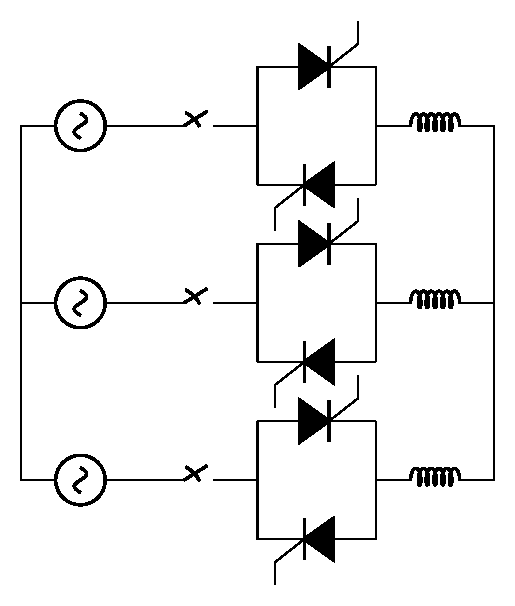
\includegraphics[width = 0.5\textwidth,angle=-90]{../sodomach/khoidongmem.pdf}
\end{center}
\end{frame}
\begin{frame}{Khởi động mềm}{Ưu điểm và ứng dụng}
\begin{itemize}
\item \alert{Ưu điểm:}
\begin{itemize}
\item Dừng tự do theo quán tính, tiết kiệm điện năng khi non tải.
\item Tránh sụt áp, tích hợp tính năng bảo vệ.
\item Điều khiển tăng tốc mịn.
\item Hạn chế dòng khởi động và điều chỉnh tăng moment mở máy.
\item \alert{Ứng dụng:} ĐC chuyên chở vật liệu, bơm, vận hành non tải, các bộ chuyển đổi, quán tính lớn,\ldots
\end{itemize}
\end{itemize}
\end{frame}
%\subsection*{Khởi động part-winding}

%--------------------------------------------------------------------------------
%--------------------------------------------------------------------------------
% Tai lieu tham khao
\section*{Tài liệu tham khảo}
\begin{frame}{Tài liệu tham khảo}
[1]. Nguyễn Văn Nhờ, \textit{Cơ sở truyền động điện}, NXB ĐH Quốc gia HCM.

[2]. Đặng Văn Đào, Lê Văn Doanh -- \textit{Kỹ thuật điện}, NXB: ĐH Khoa học và Kỹ thuật

[3]. Kênh Youtube, \textit{Phương pháp khởi động động cơ 3 pha}, \url{https://www.youtube.com/watch?v=6NdOxK7yvYo}
\end{frame}

%--------------------------------------------------------------------------------
%--------------------------------------------------------------------------------
% Tai lieu tham khao
\section*{Lời cảm ơn}
\begin{frame}
\large \alert{Cảm ơn Thầy và các bạn đã quan tâm theo dõi phần trình bày của nhóm!}
\end{frame}
\end{document}